\section{Architecture overview}

The ABEL library can be splitted into a Frontend and a Backend part.
The frontend provides the main API, which is completely agnostic of the actual storage engine, 
whereas the backend provides a framework and some implementations to adapt ABEL to a specific storage engine.
The boundary between Backend and Frontend can be drawn straight through the deferred class REPOSITORY.

\subsection{Frontend}

If you've read the previos part of the documentation, then you should be quite familiar now with the frontend.
The main classes are:
 \begin{itemize}
  \item CRUD\_EXECUTOR: Provides features for CRUD operations, and does some error handling for transaction conflicts.
  \item QUERY: Collects information like the Criteria, Projection, and (through its generic parameter) the type of the object to be retrieved. It doesn't do anything by itself.
  \item TRANSACTION: Represents an ABEL transaction, and is responsible to internally propagate errors. It provides the features commit and rollback, but internally it relies on REPOSITORY to execute them.
  \item CRITERION: Its descendants provide a filtering function for retrieved objects, and it has builtin functions to generate a tree of criteria using the overloaded logical operators.
 \end{itemize}

You can see that the main objective of the frontend is to provide an easy to use, backend-agnostic API, and to collect information that the backend can consume.

\todo{Insert class diagram}


\subsection{Backend}

The frontend needs a repository which is specific to a data storage engine, and the backend provides a framework to implement these repositories (in cluster Framework).
There are also some already predefined repositories inside the backend (cluster Backends), like the IN\_MEMORY\_REPOSITORY.

\subsubsection{The backend layers}

The framework is built of several layers, each layer more specific to a persistence mechanism as it goes down.

The uppermost layer is the REPOSITORY class. 
It provides a very high level of abstraction which should be sufficient for all kinds of persistence mechanisms.
It deals with normal Eiffel objects that may reference a lot of other objects.

One level below you can find the object-relational mapping layer.
It is responsible to take an object graph apart into its pieces and generate a plan for the write operations.
On the other hand it is responsible to build an object graph from its pieces during object retrieval.
This layer is described more precisely in the next section ~\ref{section:ORM}.

On the next level there is the BACKEND\_STRATEGY layer.
It is responsible to map the object pieces generated before to a specific storage engine, e.g. a database with some table layout.

The lowest level of abstraction is only significant for databases that can understand SQL. 
It provides a set of wrapper classes that hide connection details and error handling and has a features to execute SQL and retrieve the result in a standardized way.

\subsubsection{Important data structures}

The key data structure in the framework is the OBJECT\_\-IDENTIFICATION\_MANAGER: 
It maintains a weak reference to every object that has been queried or inserted before, and assigns a repository-wide unique number to it (called the object\_identifier).
It is, for example, responsible for the fact that the update fails in section ``Recognizing Objects''~\ref{subsection:recognize_objects}.

Another important datastructure is the KEY\_POID\_TABLE, which maps the objects object\_identifier to the primary key of the corresponding entry in the database.

\subsubsection{Transactions}

Although not directly visible, transactions play an important role in the backend.
Every operation internally runs in a backend, and almost every part in the backend is aware of transactions.
For example, the two important data structures described above have to provide some kind of rollback mechanism, and ideally all ACID properties as well.

Another important task of transactions is error propagation within the backend.
If for example an SQL statement fails because of some integrity constraint violation, then the database wrapper can set the error field in the current transaction instance and raise an exception.
As the exception propagates upwards, every layer in the backend can do the appropriate steps to bring the library back in a consistent state, using the transaction with the error inside to decide on actions.

\subsubsection{Class diagram}

To visualize the whole structure, there is a class diagram that shows the most important classes and concepts. 
You can also see two implementations of the backend abstraction there.

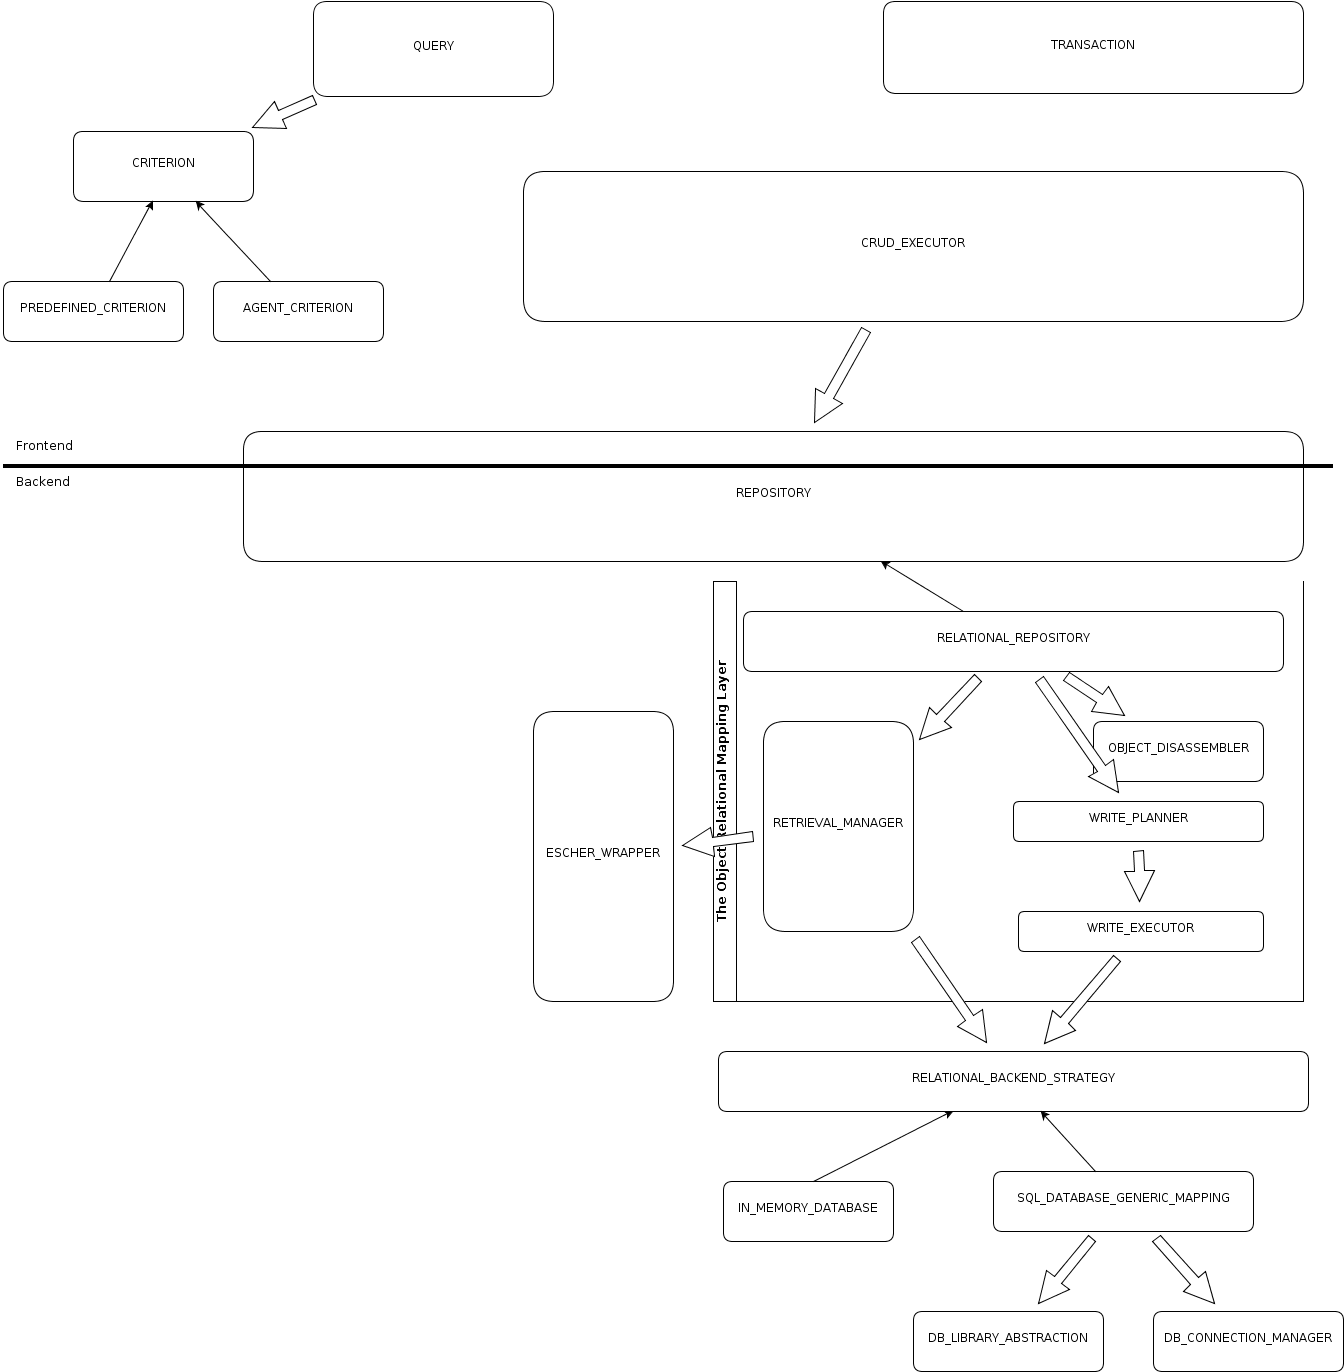
\includegraphics[width = 13cm] {class_diagram.png}

\section{Object-relational Mapping}
\label{section:ORM}

The object-relational mapping layer lies between the REPOSITORY and the BACKEND\_STRATEGY layer.
It mainly consists of four main classes doing the actual work, and a set of helper classes that represent an object graph.

The object graph representation classes are all in folder ``framework/object\_graph\_representation''. 
Although their main purpose is to represent an object graph, they are also used to describe a write operation (the BACKEND\_STRATEGY actually takes such objects as an argument)
These are the most important ones:

\begin{itemize}
 \item BASIC\_ATTRIBUTE\_PART represents an object of a basic type
 \item COLLECTION\_PART represents a collection, e.g. an instance of SPECIAL.
 \item SINGLE\_OBJECT\_PART: represets an Eiffel object that is neither a basic type nor a collection.
\end{itemize}

All these classes inherit from a deferred class OBJECT\_GRAPH\_PART. 
They have a builtin iteration cursor, and they share the concept of a dependency.

If an object graph part X is dependent on another part Y, then it means for example that Y has to be inserted first, because X needs its primary key as a foreign key in the database.

The four classes listed here are the ones that do the actual work:

\begin{itemize}
 \item The OBJECT\_DISASSEMBLER is responsible to create the explicit data structure for an object graph.
 \item The WRITE\_PLANNER is responsible to generate a total order on all write operations, taking care of the dependency relations.
 \item The RETRIEVAL\_MANAGER builds objects from the parts that it gets from the backend, and takes care that all referenced objects of a retrieved object get loaded as well.
 \item The COLLECTION\_HANDLER, or rather its descendants, add collection handling support to the basic ORM layer. 
 You need at least one handler for SPECIAL, but you can add handlers for other collection as well.
\end{itemize}

The object writing part is a bit more complex than the reading part, because of the dependency issue.


\todo{ Add a little visualization of the different parts}

\subsection{Collection handling}

You can extend the ORM algorithm to include collections. A collection is usually mapped differently from a normal object in the backend, e.g. through a M:N-relation table.
You need at least one handler for SPECIAL, because of its peculiarity that it doesn't have a fixed amount of fields.
But you can include any other collection, e.g. a LIST or an ARRAY.

There are two types of collections that you can create within a handler. 
The RELATIONAL\_COLLECTION is intended for a case when you have a typical database layout, with tables for a specific class and relations stored either with in the referenced object table (1:N-Relations) or inside their own table (M:N-Relations).
The OBJECT\_COLLECTION is intended for a scenario where you can store collections in a separate table, having their own primary key, and with the collection owner using this key as a foreign key.

Note that the choice of the collection has an effect in the object-relational mapping layer already:
\begin{itemize}
 \item An OBJECT\_COLLECTION is handled like a SINGLE\_OBJECT\_PART: The owner of the collection object depends on the collection, and the collection depends on all items that it references.
 \item A RELATIONAL\_COLLECTION in an M:N mapping mode depends on both the collection owner and all items that it references, but the owner does not depend on its collection.
 This comes from the fact that you need both a foreign key of the owner and the collection items to insert a row in a M:N-relation table
 \item A RELATIONAL\_COLLECTION in an 1:N mapping mode actually isn't forwarded to the backend at all. Instead, for each collection item there is a dependency added to the collection owner.
 Again, this comes from the normal practice in database layouts for 1:N relations.
\end{itemize}

The following diagram shows an example entity-relationship model for each type of collection:

\todo{Add model}


If you use one of the predefined backends, you usually don't have to care about collection handlers.
They become important however if you want to adapt ABEL to a custom database layout, as you can see in section ~\ref{subsection:specific_adaption}.

Please note that the framework itself does not provide any collection handler, and inserting a SPECIAL object without setting an appropriate handler will result in a runtime crash.
However, there is a SPECIAL handler shipped with the predefined backends, and e.g. the IN\_MEMORY\_REPOSITORY makes use of it.

\subsection{Object graph settings}

First, let's define the object graph more exactly, using graph theory.
A vertex in the graph corresponds to an object, and a reference is a directed edge.

The (global) object graph is the web of objects and references as it is currently in main memory.

An object Y can be ``reached'' from another object X if there is a path between X and Y, i.e. Y is in the transitive closure of X.

The object graph of an object X is an induced subgraph of the global object graph which contains all vertices that can be reached from X.

The level of an object Y in the object graph of X is the length of the shortest path from X to Y.

Using these definitions we can now describe how ABEL handles object graphs, and how you can tweak the default settings to increase performance.

Every operation in ABEL has its own depth parameter (defined in OBJECT\_GRAPH\_SETTINGS), which has the following effect:
Each operation will only handle the objects when the following condition holds: $ level(object) < depth $

Now, let's put this in a context:
You already know that the insert and retrieve features handle the complete object graph of an object. 
In fact, the depth for both functions is infinity by default.

On the other hand, the update or delete operations only handle first object they get, and don't care about the object graph.
Their depth is defined as exactly 1, which means that only an object with a level of 0 satisfies the condition above.
The only object with level 0 is in fact the root object of the object graph.

To fully understand the behaviour of ABEL, we also have to look at what happens when the algorithm reaches the ``last'' object, i.e. when the condition $level + 1 = depth$ holds.
In that case the object with all basic attributes gets inserted/updated, but references only get written if the referenced object is already persistent.
If it isn't persistent, then in a later retrieval operation the reference will be Void.

You can change the depth of the individual operations in REPOSITORY.default\_object\_graph. 
Please keep in mind that this is a dangerous operation, as a not fully retrieved or inserted object will contain Void references even in a void-safe environment, and it's also possible that they violate the invariant.

Apart from the depth, there are some other settings as well, i.e. what ABEL should do if it finds an already persistent object along the object graph of a new object to insert, or vice versa.

\section{Backend abstraction}

ABEL provides some powerful abstractions to be able to support many different storage engines. 
The three main levels of abstraction are the REPOSITORY class, the BACKEND\_STRATEGY and the database wrapper classes.

\subsection{REPOSITORY}

The deferred class REPOSITORY is the highest level of abstraction.
It deals with raw Eiffel objects and always deals with the complete object graph of such an object.
It provides a good interface for persistence mechanism that provide a similarly high level of abstraction, like for example db4o \todo{reference db4o}.

At the moment, only the RELATIONAL\_REPOSITORY implements REPOSITORY.
The RELATIONAL\_REPOSITORY uses the object-relational mapping layer and uses a generic BACKEND\_STRATEGY to perform the operations at a lower level.

\subsection{BACKEND\_STRATEGY}

The second important level of abstraction is the deferred class BACKEND\_STRATEGY.
This layer deals with one object graph part at once, either a single object or a collection.
It is responsible to map these to the actual persistence mechanism, which is usually a specific layout in a database.
Its use however is not restricted to relational databases.
The IN\_MEMORY\_DATABASE for example implements this interface to provide a fake storage engine useful for testing, and it is planned to wrap the serialization libraries using this abstraction.

\subsection{Database wrapper}


The last layer of abstraction is a set of wrappers to a database. 
It consists of three deferred classes: 
\begin{itemize}
 \item The SQL\_DATABASE\_ABSTRACTION represents a database. The main function is to acquire or release a SQL\_CONNECTION\_ABSTRACTION.
 \item The SQL\_CONNECTION\_ABSTRACTION represents a single connection. 
Its main responsibility is to forward SQL statements to the database and to represent the result in an iteration cursor of SQL\_ROW\_ABSTRACTIONs.
Another important task is to map database errors to ABEL ERROR instances.
  \item The SQL\_ROW\_ABSTRACTION represents a single row in the result of an SQL query.
\end{itemize}

The wrapper is very useful if you want to easily swap e.g. from a MySQL database to SQLite

However, keep in mind that its abstraction is not perfect. 
For example, the wrapper doesn't care about the different SQL variations, as it just forwards the statements to the database.

To overcome this problem, you can put all SQL statements in your implementation of BACKEND\_STRATEGY into a separate class and generally stick to standard SQL as much as possible.


\section{Extensions}

Due to its very flexible abstraction mechanism, you can easily extend ABEL with features like transaction management or ESCHER \todo {reference escher} integration.
The pattern how to do this is quite simple: 
You can implement a BACKEND\_STRATEGY which uses another instance of BACKEND\_STRATEGY, but does some processing on the intermediate result.
That way you can add:

\begin{itemize}
 \item Filter support for some non-persistent attributes by removing them from the OBJECT\_GRAPH\_PART during a write, and adding a default value during retrieval.
 \item ESCHER support by checking on the version attribute during a retrieval, and calling the conversion function if necessary.
 \item Client-side transaction management by using a multiversion concurrency control mechanism and delaying write operations until you can definitely commit.
 \item Caching of objects
 \item An instance that does correctness checks, e.g. by routing the calls to two different backends and comparing if the results are the same.
 \item Anything else you can imagine...
\end{itemize}

The really nice thing is that you can do that without adding complexity to the core of ABEL, and for all possible implementations of BACKEND\_STRATEGY at once.


\section{Database adaption}

The BACKEND\_STRATEGY interface allows to adapt ABEL to a lot of database layout.
Shipped with the library is a backend that uses a generic database layout which is suitable for all kinds of objects, which is explained in the next section.
But you can also adapt ABEL to your very own private database layout, as described in section ~\ref{subsection:specific_adaption}

\subsection{The generic layout backend}

The layout in the database is based upon metadata of the class. It is very flexible and allows for any type of objects to be inserted:

\todo {Add Entity-Relationship model}

In fact, this is a simplified view. 
The real model uses another relation between value and class to determine the runtime type of a value, which is required in some special cases.

The generic layout backend, located in ``backends/generic\_database\_layout'', maps Eiffel objects to this layout.

It is split into three main classes:
\begin{itemize}
 \item The METADATA\_TABLES\_MANAGER is responsible to read and write tables ``ps\_class'' and ``ps\_attribute''.
 \item The GENERIC\_LAYOUT\_SQL\_BACKEND actually implements BACKEND\_STRATEGY and is responsible to write and read the ps\_value table
 \item The GENERIC\_LAYOUT\_SQL\_STRINGS collects all SQL statements needed by the other classes. Its descendants adapt the statements to a specific database if there is an incompatibility.
\end{itemize}

The functionality of the metadata table manager is quite easy:
It just caches both metadata tables in memory and provides features to get the primary key of an attribute or a class.
If the class is not present in the database, then it will insert it and return the new primary key.

A write operation is now possible, as all required information is available: 
The attribute value in the SINGLE\_OBJECT\_PART, the attribute foreign key from the METADATA\_TABLES\_MANAGER, and the object primary key either stored in the KEY\_POID\_TABLE or generated during an insert.

The retrieval operations is similar.
You can get all attribute primary keys of a specific class from the METADATA\_TABLES\_MANAGER and then execute an SQL query which returns all values whose attribute foreign key is in the set of primary keys retrieved before, sorted by the object primary key.


\subsection{Adaption to a custom database layout}
\label{subsection:specific_adaption}

Adapting ABEL to a specific database layout needs two steps:
 \begin{itemize}
  \item Implement a BACKEND\_STRATEGY for your layout
  \item Implement COLLECTION\_HANDLERS for all collections that need to be mapped relationally
 \end{itemize}

Let's consider a very simple example. You only have two classes PERSON and ITEM:

\begin{lstlisting}[language=OOSC2Eiffel, captionpos=b, caption={Application classes}, label={lst:example_application}]
class PERSON

feature
	name:STRING

	items_owned: LINKED_LIST [ITEM]
end


class ITEM

feature
	value:INTEGER

end
\end{lstlisting}

In the database, there is table Person with columns primary\_key and name, and table Item with columns primary\_key, item, and a foreign key 'owner' to Person (as it is usual in an 1:N relation)

\todo{ER-Model}

In this setup, you only need a collection handler for LINKED\_LIST.
The collection is a RELATIONAL\_COLLECTION and it is always 1:N mapped in this simple setup.
Therefore, the implementation of your (only) collection handler is very simple:

\begin{lstlisting}[language=OOSC2Eiffel, captionpos=b, caption={The collection handler for LINKED\_LIST}, label={lst:my_linked_list_collection_handler}]
class 
	LINKED_LIST_HANDLER
inherit
	PS_COLLECTION_HANDLER [LINKED_LIST [ITEM]]
feature

	create_object_graph_part (
			obj: PS_OBJECT_IDENTIFIER_WRAPPER;
			ref_owner:PS_OBJECT_GRAPH_PART; 
			attr_name: STRING;
			mode:PS_WRITE_OPERATION)
		 : PS_RELATIONAL_COLLECTION_PART [LINKED_LIST[ITEM]]
		-- Create a new part, but don't disassemble
		do
			create Result.make (obj, ref_owner, attr_name, mode, Current)
		end

	is_in_relational_storage_mode (a_collection: PS_COLLECTION_PART[LINKED_LIST[ITEM]]):BOOLEAN = True
		-- Is `a_collection' stored in relational mode?


	is_1_to_n_mapped (a_collection:PS_COLLECTION_PART[LINKED_LIST[ITEM]]): BOOLEAN = True
		-- Is `a_collection' stored relationally in a 1:N mapping?

end
\end{lstlisting}


The implementation of BACKEND\_STRATEGY is quite straightforward as well.
You just have to distinguish between PERSON and ITEM objects and insert them in the corresponding table.

Please remember that the object-rlational mapping layer adds an attribute with name ``items\_owned'' to the ITEM object, which is the default behaviour for 1:N relations.
This especially menans that you don't need to implement the relational collection write operations.

The following code listing shows the insert feature in pseudocode:

\begin{lstlisting}[language=OOSC2Eiffel, captionpos=b, caption={The collection handler for LINKED\_LIST}, label={lst:my_backend_adaption}]
class 
	MY_SIMPLE_BACKEND
inherit
	PS_BACKEND_STRATEGY
feature

	insert (an_object:PS_SINGLE_OBJECT_PART; a_transaction:PS_TRANSACTION)
		-- Inserts the object into the database
		do
			if an_object is a PERSON object then
				database.execute_sql ("INSERT INTO person (name) VALUES " + an_object.get_value ("name"))
				key_mapper.add_entry (an_object, database.execute_sql ( "Get last autoincremented primary key of Person")
			else
				-- The ORM layer has added an attribute `items_owned' in ITEM
				foreign_key:= key_mapper.primary_key_of (an_object.get_value ("items_owned"))
				database.execute_sql ("INSERT INTO item (value, owner) VALUES " + an_object.get_value ("value") + foreign_key)
				key_mapper.add_entry (an_object, database.execute_sql ("Get last autoincremented primary key of Item")
			end
		end


	key_mapper: PS_KEY_POID_TABLE
		-- Maps object identifiers to primary keys

end
\end{lstlisting}

During a retrieval operation, you similarly have to select your values from the correct table.
Note that you need the retrieve\_relational\_collection here.


%\section{Tuning performance}

%Performance rather belongs to the future work section...


%\subsubsection{Performance remarks}

%ABEL will try to let the backend do as much of the filtering as is possible, to reduce the overhead of e.g. network communication or building unnecessary objects.
%This especially means that ABEL will compile predefined queries to SQL if you have a relational database as a backend. 
%However, if there is an agent criterion OR-ed to a predefined criterion, the test can not be made in the database because you might get false negatives.
%Therefore, to have optimal performance, you should consider the following points:

%\begin{itemize}
%\item Try not to use agent criteria if you have a relational database backend.
%\item Try not to use OR on agent criteria.
%\item Try to keep OR-ed agent criteria as deep down the tree as possible (as the above OR-node defaults to true and thus is not checked for in the backend)
%\end{itemize}
